\subsection*{Introduction to Mechanical Heart Valves}
Mechanical heart valves have been around for half a century now. Over the years, many heart valves have been designed and implanted into patients. The key positions for these implants are the aortic and mitral positions.\cite*{hutchison2011} The valves can be either fully mechanical or bioprosthetic. Depending on the target position and the patient's condition, either mechanical or bioprosthetic valves may be used. The mechanical valves are often made of stainless steel, titanium, or carbon-coated materials. These are more durable than bioprosthetic valves. The bioprosthetic valves are often made of porcine or bovine tissues integrated with stainless steel, titanium, or carbon-coated materials.\cite*{venkatesh2013} Bioprosthetic valves can be preferred in some patients when the intake of anticoagulant medication is problematic.
\\Mechanical heart valves come in different shapes and sizes. Depending on the price set by the manufacturer, or availability the choice of valves is somewhat more flexible when it comes to in situ application. Most valves used contemporarily perform well for decades after implantation even though they are mostly coupled with anticoagulation therapy throughout the patients' lives. From an engineer or materials scientist's point of view, it is important to consider the material composition and geometry of the valves more in-depth, which will be done in the next sections.\\
\subsection*{Material Composition and Structure}
The main parameters that are important in mechanical heart valves are biocompatibility, wear resistance, radioopacity, and durability. Most valves use tungsten-impregnated pyrolytic carbon over graphite, titanium coated with pyrolytic carbon, and barium-containing silastic polymer.\cite*{hutchison2011} There are more than seventy different cardiac valves available in the market, but they can be categorized under four main types. These are Caged Ball Valves, Tilting Disk Valves, Bileaflet Valves, and Bioprosthetic Valves.\cite*{venkatesh2013} Björk-Shiley valve acquired for this research proposal, is one of the most studied valves and it is a tilting disk valve. The Medtronic valve acquired for this research is a type of leaflet valve. Both valves are made of pyrolytic carbon-coated titanium alloys.

\begin{figure}
    \centering
    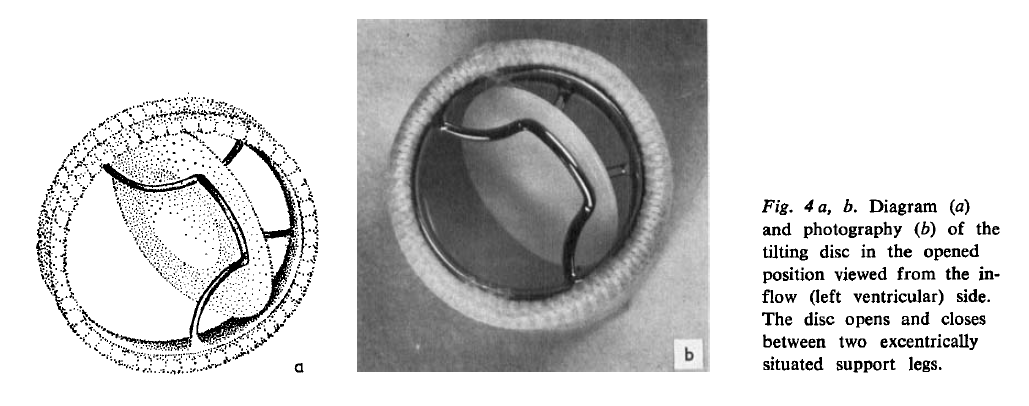
\includegraphics[width=0.8\textwidth]{björkshileyvalve.png}
    \caption{Björk-Shiley Valve. \cite*{björk1969}}
    \label{fig:björkshileyvalve}
\end{figure}
\vspace{1pt}

\subsection*{Complications}
There are some complications that arise from prosthetic heart valves. These are the growth of pannus tissue, infective endocarditis, thrombosis, and hemolysis.\cite*{roudaut2007} \cite*{barmada1998} The pannus tissue is a connective tissue that grows onto the heart valves eventually hindering its movement. Infective endocarditis is a medical issue that usually occurs as a result of the bacterial infection of the heart valve and the surrounding tissue triggered by the cardiologic/surgical operation. The last two issues, however, are more related to the surface quality and structural integrity of the mechanical heart valves. The roughened surface of the valve provides a more suitable environment for thrombosis to occur, increasing the risk of blood clot formation. Furthermore, the presence of microcracks in the valve structure can contribute to the formation of thrombosis and also compromise the durability of the prosthetic. In some extreme cases, the formation and propagation of microcracks can reach such a level that the leaflet/leaflets of the heart valve break off and cause complete valve failure, causing significant problems by embolization in the arterial tree.\cite*{vansteenbergen2019}
\subsection*{Methods of Detecting and Monitoring Microcracks}
There are several methods to detect the presence of faults in the heart valves. Some of these methods are echocardiography, cardiac tomography, x-ray examination, fluoroscopy, or suspicion raised from certain patient symptoms similar to heart valve disease like shortness of breath, feeling dizzy and tired, etc. Medical professionals can also use a stethoscope to listen to the sound of the heart valves and detect a decrease in the valve sound, which would mean reduced functionality. The most extensive way, however, is only possible after the removal of the mechanical heart valves and inspection under a light microscope (LM), where the presence and extent of microcracks can be visually examined, later scanning electron microscopy (SEM) and possibly even fringe pattern interferometry (FPI).\cite*{barmada1998} FPI will give insight into the roughness of the surface.

\subsection*{Common causes of Microcracks}
Microcracks and other surface defects on the valves arise after years of operation. Certain parameters in the body like pressure inside the veins, repeated load, and friction can contribute to the formation and progression of microcracks in mechanical heart valves. One of the important phenomena that add to surface defects and microcracks is the cavitation potential of the blood.\cite*{zhang1995} This is observed when the local pressure of the blood drops below the vapor pressure, causing the rapid formation of bubbles that implodes upon reaching areas of higher pressure. This causes shock waves on nearby surfaces, in this case, the surface of the mechanical heart valve.\cite*{wu2001} These shock waves contribute to the formation of microcracks and erosion of the surface of the valves.

